\documentclass[american,12pt]{article}

\usepackage[utf8]{inputenc}
\usepackage[T1]{fontenc}
\usepackage{hyperref}
\usepackage{babel}
\usepackage{csquotes}
\usepackage[backend=biber,date=short,maxcitenames=2,style=apa]{biblatex}
\usepackage{enumitem}
\usepackage{tikz}
\usepackage[margin=1in]{geometry}
\usepackage{graphicx}

\DeclareGraphicsExtensions{.png,.jpg,.pdf,.eps}

\usetikzlibrary{patterns,fit,positioning}

\DeclareLanguageMapping{american}{american-apa}

\title{Automated Aquaponics Developer Setup Manual}
\author{Henry J Schmale}
\date{\today}

\addbibresource{project.bib}
\nocite{*}

\begin{document}
\maketitle
\tableofcontents
\listoffigures

\newpage

\section{Introduction}
This manual provides the documentation for my partially automated aquaponics
system. The system provides facilities for monitoring fish count, water level,
water temperature, and air quality factors. It also provides control systems
for toggling the pumps on and off, along with lighting factors for the tank.

\section{System Architecture}
The control system consists of many parts, such as the database, data collection
and control, and web interface. The database provides storage of the various
events and readings collected. The web interface provides control of the various
components to the user, and allows the user to view the current status of the system.
The data and control system manages the connection to the microcontroller, and collects
data from the various sensors, it also manages the toggling of the various pumps and
lights to keep the fish alive.

\begin{figure}[h]
    \centering
    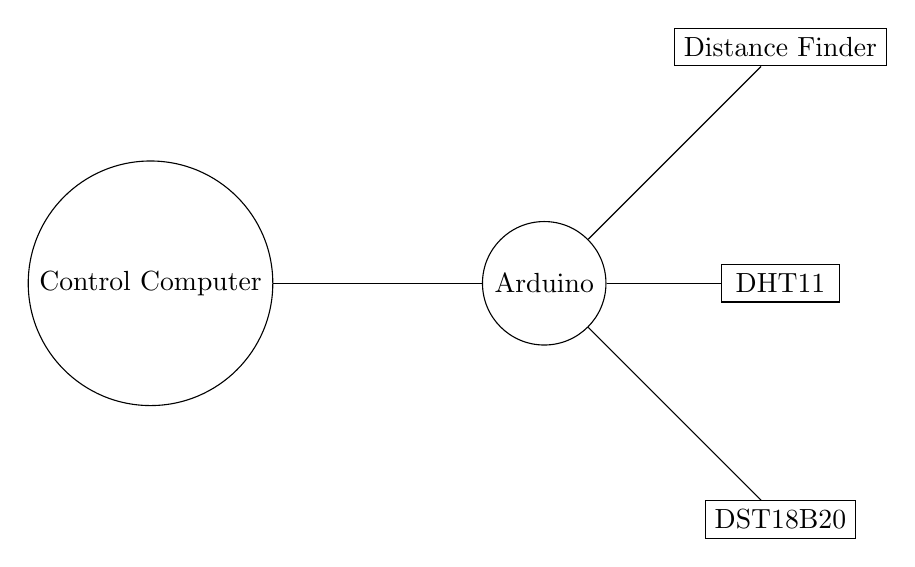
\begin{tikzpicture}[
            every node/.style={circle,minimum width=15mm,draw}
        ]
        \node (a) at (0,0)             {Control Computer};
        \node (b) at (5,0)             {Arduino};
        \node[rectangle] (c) at (8,-3) {DST18B20};
        \node[rectangle] (d) at (8,0)  {DHT11};
        \node[rectangle] (e) at (8,3)  {Distance Finder};

        \draw (a) -- (b);
        \draw (b) -- (c);
        \draw (b) -- (d);
        \draw (b) -- (e);
    \end{tikzpicture}
    \caption{The Hardware Architecture and Sensor Connections}
    \label{fig:Hardware Architecture}
\end{figure}

There are 3 main parts in the automated aquaponics system, database,
web app, and control daemon. The web app provides details of the current
system state over time, scheduling of actions, and the ability to edit
minor configuration settings. The control daemon requests sensor readings,
updates the relay configuration, and manages the communication between the
control board and the database. The final piece of the puzzle is the
database, it manages communication between the web app and control daemon in
a structured method. The data flow between the daemons can be seen in 
fig~\ref{fig:Software Architecture}.

\begin{figure}[h]
    \centering
    
\begin{tikzpicture}
        \node (a) {R Shiny Web App};
        \node[right=of a] (b) {SQLite Database};
        \node[right=of b] (c) {Control and Management Daemon};
        \node[below=of c] (e) {Arduino};

        \draw[<->] (a) -- (b);
        \draw[<->] (b) -- (c);
        \draw[<->,dashed] (c) -- (e);
    \end{tikzpicture}
    \caption{The software daemons and connections}
    \label{fig:Software Architecture}
\end{figure}

\subsection{Database}
There is a database meant to facilitate communication between each of the 
process segments. 

\subsection{The Web App}
The web app is written using the shiny R framework. This framework allows for 
analytic dashboard apps to be built quickly and efficiently. It connects to
the database using the DBI package, which allows for powerful reporting, and
quick inserts. It also uses the shinydashboard package to provide a very
pretty dashboard experience.

There are three tabs in the interface. The first tab provides detailed
analytics of the system, and current stats about the system. The second
tab provides a scheduling interface that allows for the various pumps
and lights to be switched on and off. The final tab allows for 
configuring the constraints that will trigger a warning to be sent to
the operator.

The general stats tab is the first thing viewed when the web interface is
pulled up, see fig~\ref{fig:data dashboard}. It provides the most recent 
readings from the system, and
graphs that show the changes over time for each of the monitored sensors.
The interactivity of the graphs is provided by the "plot.ly" package.

\begin{figure}[h]
	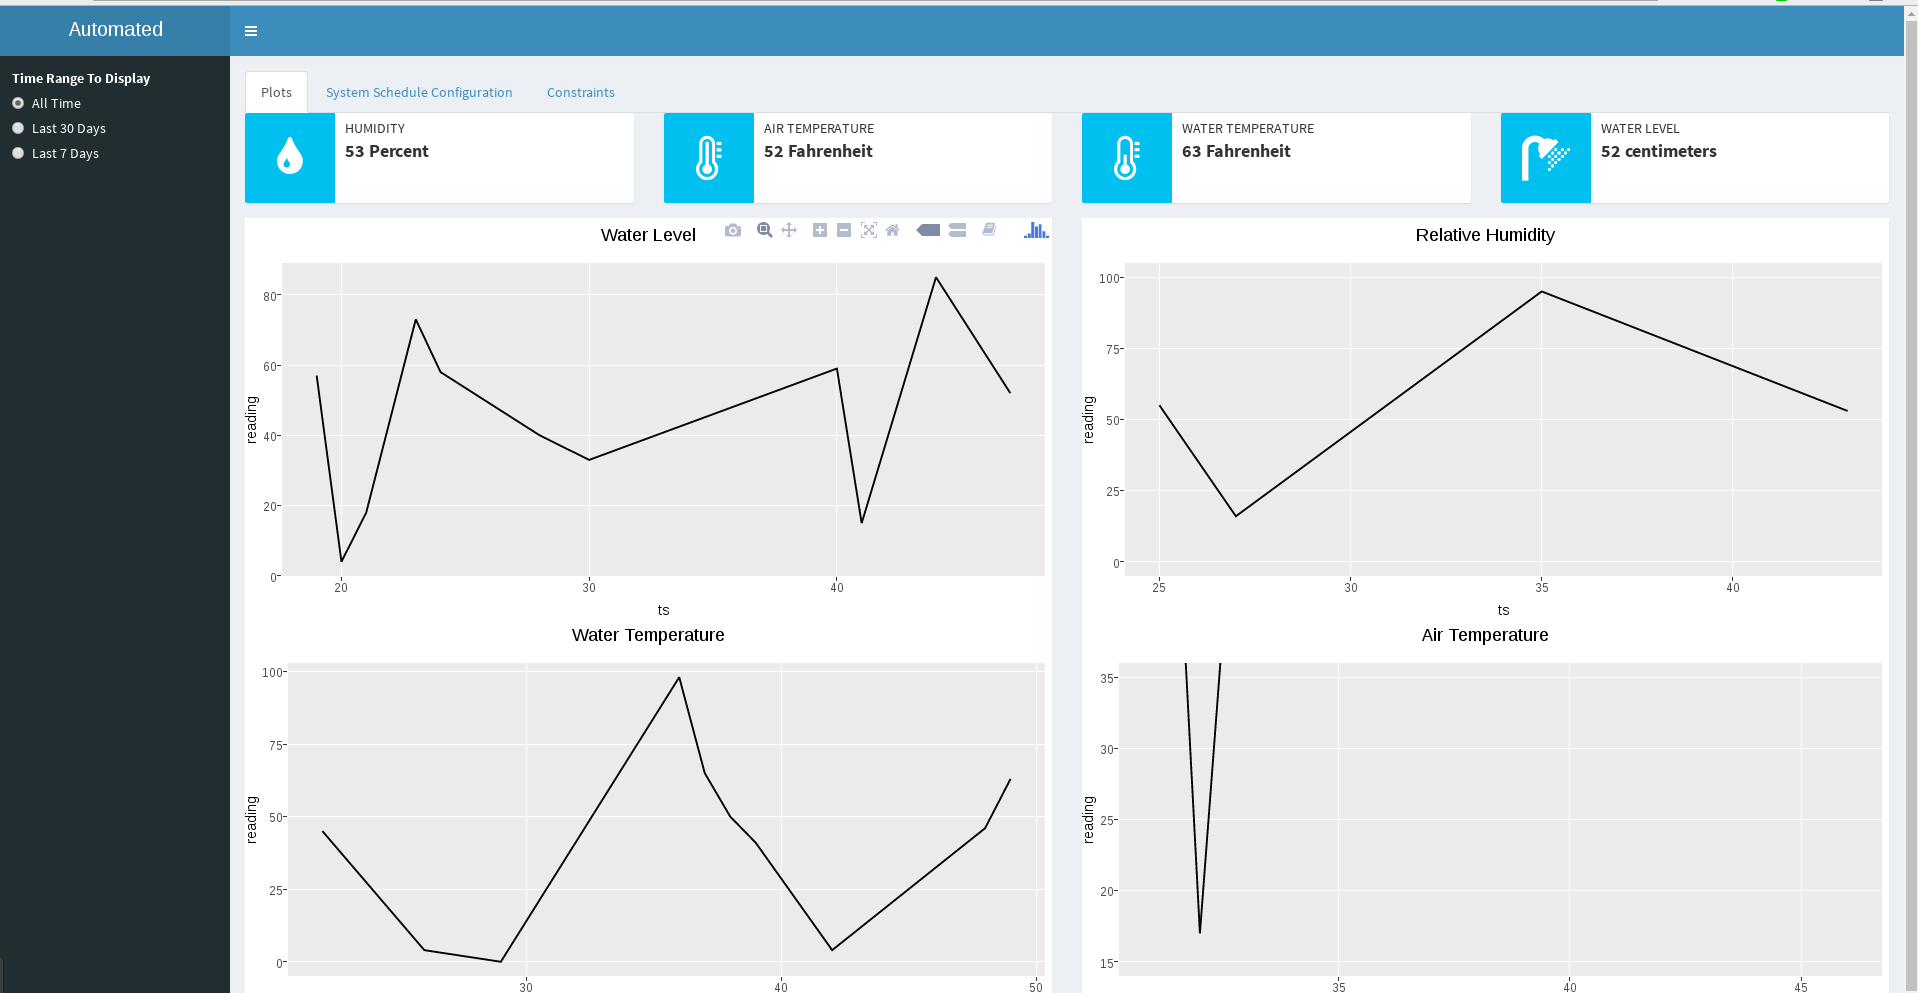
\includegraphics[width=\linewidth]{imgs/WebappDashboard}
	\label{fig:data dashboard}
	\caption{The dashboard with some test data placed in it.}
\end{figure}

The scheduling interface is based off of the parental controls interface
in windows 7 for allowing users to have access during set times. The blue
boxes represent the times that it is on, and the white boxes represent the
times that it is off. The scheduling interface can be viewed in
fig~\ref{fig:schedular}.

\begin{figure}[h]
	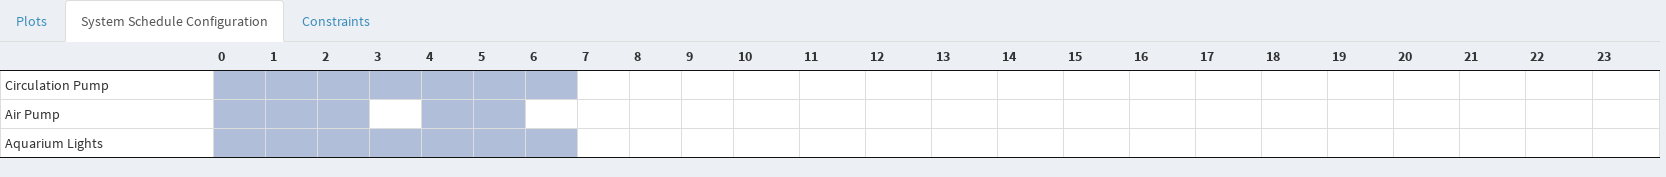
\includegraphics[width=\linewidth]{imgs/sched}
	\label{fig:schedular}
	\caption{The scheduling interface for the pumps and lights}
\end{figure}

The final interface is the constraint configuration manager,
see fig~\ref{fig:constraints}. 
This interface allows
one to set the points at which a warning message is sent to the operator.
It provides constraints for three sensor values: air and water temperature,
and water level. The changes are not automatically committed to the database,
the "save constraints" button must be clicked.

\begin{figure}[h]
	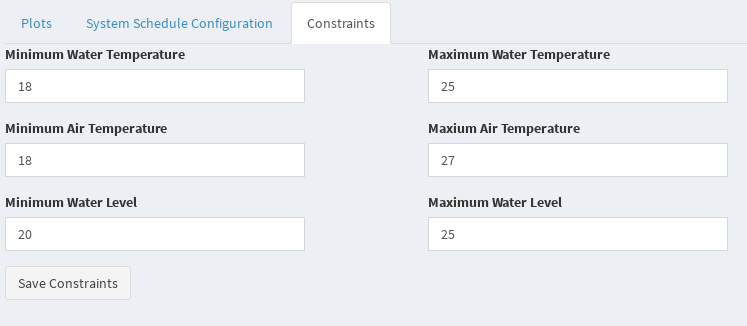
\includegraphics[width=\linewidth]{imgs/constraints}
	\label{fig:constraints}
	\caption{The constraint configuration manager tab}
\end{figure}

\subsection{Serial Communication Protocol}
This section describes the command protocol used to communicate with the
microcontroller over serial. The protocol is that of a client and server,
with line delimitation. The first step is for the client, in this case the
main computer, to send a command in the list of known commands. The server,
arduino, receives the command and performs the action. Over the same link, it
will send back the command and the value returned separated by a space. By
duplicating the command it allows multiple commands to be queued over the same
link, without worry of the data being muddled.

\begin{description}[style=nextline]
    \item[rWatThm] read the water thermometer
    \item[rdWaLvl] read the distance measuring device to obtain distance to water.
    \item[rdHumid] read the current humidity in the room
    \item[rdAirTm] read the current air temperature
\end{description}

The below commands affect the switching of various components. They are set by
prepending a 'y' or 'n' respectively to switch it on and off.

\begin{description}[style=nextline]
    \item[CiPump] switches the circulation pump
    \item[Lights] switches the lights
    \item[AirPmp] switches the air pump
\end{description}




\subsection{Sensors}
This section describes the various sensors used to monitor the system, and their
purpose. These sensors include temperature probes, distance measuring devices,
and humidity. These sensors allow the user to correlate the data with how well
their fish are doing.

\subsubsection{Water Level with Distance Measuring}
The depth of the water is measured using an ultrasonic distance sensor. It uses
sound to find how distant an object is, in this case the surface of the water.
This method assumes that the total distance between the sensor and the container
bottom is known as $D_t$, and the distance between the water surface and the sensor
is known as $D_a$. The water depth is then obtained using the following formula,
$D_w = D_t - D_a$. Please see figure~\ref{fig:distance measuring} for details on the
measurement.

\begin{figure}[h]
    \centering
    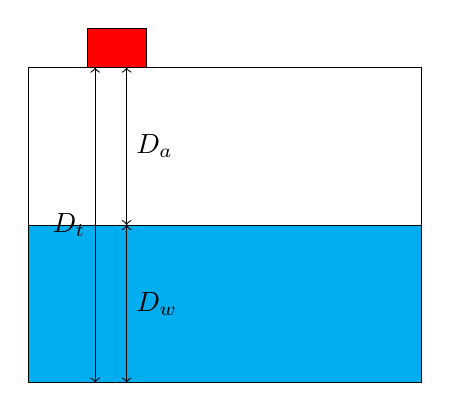
\begin{tikzpicture}
        \draw[fill=red] (0.75,4) rectangle (1.5,4.5);
        \draw (0,0) rectangle (5, 4);
        \draw[fill=cyan](0,0) rectangle (5,2);
        % dim lines
        \draw[<->,black] (.85,0) -- node[left]{$D_t$}  (.85,4);
        \draw[<->,black] (1.25,0) -- node[right]{$D_{w}$} (1.25,2);
        \draw[<->,black] (1.25,2) -- node[right]{$D_{a}$} (1.25,4);
    \end{tikzpicture}
    \caption{How the distance measuring works}
    \label{fig:distance measuring}
\end{figure}

\subsubsection{Air Temperature and Humidity}
The air temperature and humidity is obtained using a DHT series sensor. It can
use any sensor in this series so long as the code on the microcontroller is
updated. The Adafruit Unified Sensor library is used with DHT extension to
perform this interfacing on the
microcontroller(\cite{adafruit-unified-sensor,adafruit-dht}). The current system
uses the DHT11 sensor, as this was the most common sensor available at build
time.

\subsubsection{Water Temperature}
The measurement of water temperature is carried out using Dallas Temperature
Probe. This sensor is interfaced using the Maxim Temperature Integrated Circuit
Library (\cite{gh-arduino-temperature}). The current system uses
a DST18B20 sensor.

\section{Parts List}
\begin{itemize}
    \item Large Plastic Reservoir.
    \item 3 inch PVC Pipe, 5 foot long.
    \item Net Pots
    \item 390 Gallon Per Hour Submersible Pump
    \item 2 - 1/2 inch hose barbs threaded
    \item Hose Clamps
    \item GFCI Outlet
    \item Regular Outlets
    \item Arduino Mega
\end{itemize}

\section{Diagram}
Please see figure~\ref{fig:views} for a limited drawing of the system.
Due to the way the apa6 package works the
diagrams must be referenced and cannot be placed here, but are at the end. These
diagrams are not to scale, and are not absolute as the number of holes may vary
and the dimensions are up to the user. They are to give a general idea of a
finished system.

\begin{figure}[h]
    \centering
    % front view
    \begin{tikzpicture}
        \draw (0,0) rectangle (6, 4);
        \draw (0,4) -- (.25,4.25) -- (5.75,4.25) -- (6,4);
        % pipe
        \draw (-1,4.25) rectangle (7,4.75);
        \foreach \x in {-.5,0,.5,1,1.5,2,2.5,3,3.5,4,4.5,5,5.5,6}
        \draw (\x,4.75) arc (230:310:.3);
    \end{tikzpicture}
    % top view
    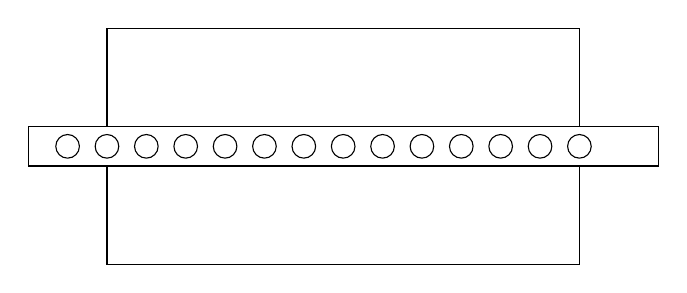
\begin{tikzpicture}
        \draw (0,0) rectangle (6, 3);
        % the pipe
        \draw[fill=white] (-1,1.25) rectangle (7,1.75);
        \foreach \x in {-.5,0,.5,1,1.5,2,2.5,3,3.5,4,4.5,5,5.5,6}
        \draw (\x,1.5) circle [radius=.15];
    \end{tikzpicture}
    \caption{Various Views of the Test System Container. Front view left, Top
    view right}
    \label{fig:views}
\end{figure}

\section{How To Build}
\begin{enumerate}
    \item Drill PVC pipe with hole saw. Start placing holes 7 inches from the
        end, and then 6 inches on center. Continue until you have reached
        the end of the pipe, but still have about 7 inches.
    \item Drill holes into each of the end caps slightly off center.
    \item Place the hose barb fittings into the holes that you drilled.
    \item Glue the end caps to the pipe in such a way that there is a difference
   	      in heights between the two holes. The lower hole should be the drain
   	      hole.
   	\item Place holes in the reservoir to run the hose lines, and sensors.
   	\item The electrical work is classified as of right now even though anybody
   	      could figure it out.
\end{enumerate}


\section{Starting a new garden}
This section describes how to start a new crop in the automated aquaponics
system. It is broken down into two sections, the fish and starting the plants.
This section is still under construction.

\begin{enumerate}
    \item Fill tank with water.
    \item Start pump circulation.
    \item Introduce the fish to the system.
    \item Start plants in the rockwool plugs.
\end{enumerate}

\section{Troubleshooting}
This section describes various problems that might occur in the 
aquaponics system and how to resolve them. This section is still
being expanded as problems arise in the test system and
resolved.

\begin{itemize}
	\item Grow Pipe Not Draining
	\begin{enumerate}
		\item Check that drain hose is elevated out of water.
		\item Check that flow rate into pipe is low enough that it can still 
			drain. Install a valve on to pump input line to reduce the flow 
			rate.
	\end{enumerate}
\end{itemize}

\newpage
\printbibliography
\end{document}
